\chapter{Programming interpreters}
\label{meta}

\index{meta programming techniques}
\lettrine[nindent=0.1em]{A}{number of programming techniques} rely on or can be considered to be variations of \firstterm{meta programming}{A style of programming that leverages the relationship between the name or description of an entity and the entity itself. A common use of meta-programming is the \emph{interpreter}; which is a program that interprets a data structure that represents a program, allowing computation with that represented program. Another common example is the use of `class of' operators that allow introspection of objects.}. Meta programming is a style of programming that leverages the relationship between the name or description of an entity and the entity itself. A common meta-programming example is the interpreter; which is a program that interprets a data structure that represents a program, allowing computation with that represented program. Another common example is the use of `class of' operators that allow introspection of objects. In this chapter we explore how to build an \emph{interpreter} for a very simple logic-like language in \go.

\section{A simple logic language}
Our simple logic language is a variant of horn-clause logic: a program consists of clauses, each clause is of the form of a `body' and a `head'; the interpretation of this being that if the body is satisfied then the head is also satisfied. 

Note that since \go is a strongly typed language, we would like to extend this also to our interpreted language. I.e., even though our language is intended to be interpreted, for it to integrate smoothly with \go it is necessary to be equally rigorous about types. We can do this and still maintain generality by using different classes to implement the different kinds of logical formulae, all sharing a common type -- \q{metaTp}.

\subsection{Representing language elements}
\index{representing logical formulae}
\label{meta:type}
In order to interpret a data structure as a language we need to \emph{represent} elements of the language as \go structures. In the case of our logic language we need to be able to represent rules, conditions, terms and so on. One way of doing this could be to use constructors for each of possible elements, for example to use a term
\begin{alltt}
conj([ C\sub1, \ldots, C\subn])
\end{alltt}
to represent a conjunction. The definition of these constructors might take the form of a algebraic type definition:
\begin{alltt}
metaTp[CT] ::=  conj(list[metaTp[CT]]) | \ldots
\end{alltt}
A slightly more paradigmatic approach is to define an \emph{interface} for rules and conditions, and then to define classes that implement the interface. In the case of a condition, the immediate interface requirement is to be able to \emph{evaluate} the condition; in the case of a logic language evaluation is expressed primarily as \q{satisfy} -- solving queries. We detail this interface in program~\ref{meta:interface}.
\begin{program}
\vspace{0.5ex}
\begin{alltt}
meta\{
  metaTp \impl \{ satisfy:[]\{\} \}.
  ...
\}
\end{alltt}
\vspace{-2ex}
\caption{The interpreter interface}
\label{meta:interface}
\end{program}

With this type interface we can begin to define classes that implement the \q{metaTp} interface. For example, the \q{conj} class is detailed in program~\vref{meta:conj}.
\begin{program}
\vspace{0.5ex}
\begin{alltt}
conj:[list[metaTp]]\conarrow{}metaTp.
conj(C)..\{
  satisfy() :-
    solve(C).
  
  solve:[list[metaTp]]\{\}.
  solve([]).
  solve([G,..R]) :- G.satisfy(), solve(R).
\}
\end{alltt}
\vspace{-2ex}
\caption{The \q{conj} class}
\label{meta:conj}
\end{program}
An interesting feature of \q{satisfy} in the definition of \q{conj} is that it uses the label argument \q{C} from the class label to \emph{carry} the data. We can see this if we look at a typical call to \q{satisfy} using a \q{conj} label:
\begin{alltt}
conj([\emph{C\sub1},\ldots,\emph{C\subn}]).satisfy()
\end{alltt}
The list of \emph{C\subi} represents conditions to satisfy; within the \q{conj} class these conditions are held in the label argument \q{C}. Of course, this is just how one might use \prolog terms to represent interpreted programs. However, \prolog cannot easily combine this with the invocation of programs the way that we can use classes in \go.

The class definitions for the disjunctive case -- \q{disj} -- and negation -- \q{not} -- are directly analogous to the \q{conj} class. The only difference is in the definitions of \q{satisfy} within each class. Program~\vref{meta:disnot} contains, for reference, these classes.
\begin{program}
\vspace{0.5ex}
\begin{alltt}
disj:[list[metaTp]]\conarrow{}metaTp.
disj(C)..\{
  satisfy() :-
    G in C, G.satisfy().
\}.

not:[metaTp]\conarrow{}metaTp.
not(C)..\{
  satisfy() :-
    \nasf{} C.satisfy().
\}
\end{alltt}
\vspace{-2ex}
\caption{Disjunction and negation}
\label{meta:disnot}
\end{program}

The class for implementing rules is not a great deal more complex than those for the query types. The main technique required is to represent calls to interpreted rule programs with their class label -- \q{ask} -- in our version; and to rely on a repository for the rules themselves.
\begin{program}
\vspace{0.5ex}
\begin{alltt}
ask:[metaTp]\conarrow{}metaTp.
ask(P)..\{
  satisfy() :-
    isRule(P,Body),
    Body.satisfy().
\}.
\end{alltt}
\vspace{-2ex}
\caption{Interpreted rules}
\label{meta:rule}
\end{program}
The \q{isRule} relation mentioned in program~\vref{meta:rule} represents the main repository of interpreted rules. Given that we are interpreting programs, it is likely that this repository is itself represented using \q{dynamic} relations which we have already seen used to store descriptions in a directory in program~\vref{directory:directory}. 

\subsection{Escaping into regular \go}
An interpreter for any language has to handle two fundamental aspects of the language: how composite elements are interpreted -- in our case these are disjunction, conjunction and so on -- and how primitive elements are interpreted. These primitive elements may be like \emph{escapes} -- that invoke functionality directly from \go.\note{The \go engine itself has escapes that invoke ``C'' code for executing operating system functions such as reading and writing to files.}

Our escape technique reflects the inherent extensibility of \go's object oriented system. All that is really required is that each primitive is represented by a class that realizes the \q{metaTp} type. We illustrate this in program~\vref{meta:plus} with a pseudo-logical primitive -- \q{plus} -- which implements arithmetic.
\begin{program}
\vspace{0.5ex}
\begin{alltt}
plus:[integer, integer, integer]\conarrow{}metaTp.
plus(A,B,C)..\{
  satisfy() :-
    C = A+B.
\}.
\end{alltt}
\vspace{-2ex}
\caption{Intepreted addition}
\label{meta:plus}
\end{program}

We can use a \q{plus} condition in a query in much the same way as we would use a \q{conj} condition, the main difference being that the arguments of \q{plus} are numeric:
\begin{alltt}
conj([plus(1,2,x),conj([plus(2,1,x)])]).satisfy()
\end{alltt}

\section{Dynamic family relationships}
\label{meta:family}
If we were representing -- in \go -- some simple genealogical relations between people, such as who is the parent of who, then we might expect to be able to use rules such as
\begin{alltt}
parent:[symbol,symbol]\{\}
parent('j','k').
parent('k','l').
\end{alltt}
We have some flexibility in how we represent such data so that our interpreter system can reason genealogically. We could, for example, throw everything into a single \q{dynamic} relation and fetch individual facts as needed. However, that seems clumsy.

\subsection{Dynamic relations}
\index{representing dynamic relations}
One effective of incorporating dynamic relations into our interpreted system is to use a \emph{paired} approach -- to construct a pair consisting of a \q{parent} class with the normal \q{metaTp} type interface, and a separate parallel \q{Parent} entity that realizes a \q{dynRel} type that supports an \q{assert} interface.\note{The \q{mailbox[]}/\q{dropbox[]} pair in the \q{go.mbox} package -- discussed in Section~\vref{dance:mbox} -- is another example of this kind of pairing.}

Program~\vref{meta:ppackage} shows an example of this for the \q{parent} relation and its \q{Parent} paired \q{dynamic} set.

\begin{program}
\vspace{0.5ex}
\begin{alltt}
parent\{
  import meta.
  import dynamicRel.
  
  Parent:dynRel[(symbol,symbol)] = dynRel([]).
  
  parent:[symbol,symbol]\conarrow{}metaTp.
  parent(A,B)..\{
    satisfy() :-
      Parent.mem((A,B)).
  \}.
\}.
\end{alltt}
\vspace{-2ex}
\caption{Parent package}
\label{meta:ppackage}
\end{program}

To query the \q{parent} relation, we use the same queries as for non-dynamic relations:
\begin{alltt}
parent('jim','bill').satisfy()
\end{alltt}
to represent queries to the \q{parent} relation.
To modify the relation, perhaps to record a new birth, we use actions of the form:
\begin{alltt}
Parent.assert(('jim','joe'))
\end{alltt}

\begin{aside}
Note that, although, in program~\vref{meta:ppackage}, we can modify the \q{parent} relation -- through the \q{assert} and \q{retract} methods on the associated \q{Parent} --  this is still not the same as \prolog's assert and retract primitives.

The reason is that our interpreted rules cannot invoke these methods as part of the query evaluation. Of course, the application in which the meta-system is embedded can modify the dynamic relations. This separation is enough to ensure logical soundness of the interpreter -- assuming that the main query evaluation procedure is sound.
\end{aside}

The \q{dynamicRel} class is a straightforward use of the \q{dynamic} class, and is shown in Program~\vref{meta:dynamic}.

\begin{program}
\vspace{0.5ex}
\begin{alltt}
dynamicRel\{
  import go.dynamic.

  dynRel[T] \impl{} \{ assert:[T]*. retract:[T]* \}.
  dynRel[T] \impl{} dynamic[T].

  dynamicRel:[list[T]]\sconarrow{}dynRel[T].
  dynamicRel(I) <= dynamic(I).
  dynamicRel(_)..\{
    assert(X) ->
        add(X).
    retract(X) ->
    	    del(X).
  \}.
\}.
\end{alltt}
\vspace{-2ex}
\caption{Dynamic interpreted relations}
\label{meta:dynamic}
\end{program}

\subsection{Family ancestors}
\label{meta:ancestor}
Not all interpreted relations are \emph{flat} -- some are better expressed as recursive rules. For example, the ancestor relation might be defined in regular \go as:
\begin{alltt}
ancestor:[symbol,symbol]\{\}.
ancestor(X,Y) :- parent(X,Y).
ancestor(X,Y) :- parent(X,Z), ancestor(Z,Y).
\end{alltt}
We could incorporate such a recursive rule into our interpreted system in the same way that we incorporated \q{plus} in Program~\vref{meta:plus}. However, we can also \emph{interpret} ancestors; supporting dynamic rules in an analogous way that we supported dynamic relations. 

\begin{program}[bt]
\vspace{0.5ex}
\begin{alltt}
dynamicRules\{
  import go.dynamic.
  import meta.

  dynRule[T] \impl \{ assert:[T,metaTp]*. satisfy:[T]\{\} \}.
  dynRule[T] \impl dynamic[T].

  dynamicRule:[list[T]]\sconarrow{}dynRule[T].
  dynamicRule(I) <= dynamic(I).
  dynamicRule(_)..\{
    satisfy(X) :-
        mem((X,B)),
        B.satisfy().
    assert(X,B) ->
        add((X,B)).
  \}.
\}.
\end{alltt}
\vspace{-2ex}
\caption{Interpreted rules}
\label{meta:rules}
\end{program}

Program~\vref{meta:rules} is a package that is similar to the package in Program~\vref{meta:dynamic}; oriented to handling rules. Like that program, we define a new interface for handling dynamic rule programs. The \q{dynRule[]} type has a \q{satisfy} element, as well as an \q{assert} element to simplify the paired rule programs. 

\begin{program}[bt]
\vspace{0.5ex}
\begin{alltt}
ancestor\{
  import meta.
  import dynamicRules.
  import parent.

  Ancestor:dynRule[(symbol,symbol)]=
      dynamicRule([((A,B),parent(A,B)),
                   ((A,C),conj([parent(A,B),
                                ancestor(B,C)]))]).

  ancestor:[symbol,symbol]\conarrow{}metaTp.
  ancestor(A,B)..\{
    satisfy() :- Ancestor.satisfy((A,B)).
  \}.
\}
\end{alltt}
\vspace{-2ex}
\caption{Interpreted ancestry}
\label{meta:dynamic:ancestor}
\end{program}

The \q{satisfy} relation definition in the \q{dynamicRule} class uses \q{mem} to find a rule -- represented as a pair consisting of a head and a body. The body is a \q{metaTp} term, which is queried by invoking \q{satisfy} on that term. 

The definition of \q{ancestor} in program~\vref{meta:dynamic:ancestor} shows how we can use the \q{dynamicRule} class to establish the rules of ancestry.

\index{variable!in \q{dyamic} relations}
\index{dynamic@\q{dynamic} relation!variables in}
A sharp observer might wonder how \emph{variables} are managed in the representation of the rules for \q{ancestor}. Normally, assignable values are required to be \emph{ground}; which clearly will not permit us to represent rules such as for ancestor. However, the \q{dynamicRules} package relies on the standard \q{go.dynamic} package. This package implements a subtly different semantics for assignment.

In a \q{dynamic} relation, the entries are generally tuples. When a tuple has one or more variables in it then, whenever that tuple is retrieved from the \q{dynamic} relation -- typically by way of the \q{mem} predicate method -- the variables in the tuple are \emph{refreshed} each time. That means that the tuple is \emph{copied} and any variables replaced with new ones. Thus each time a tuple is retrieved from the \q{dynamic} relation, it will have different variables in it. 

This refreshment, which in logic is called \emph{standardizing apart}, is how we are able to use a \q{dynamic} relation to store the rules for the recursive \q{ancestor} program without getting the variables in it confused.

\section{Family trees}
\label{meta:family:tree}

\begin{figure}[bt]
\centerline{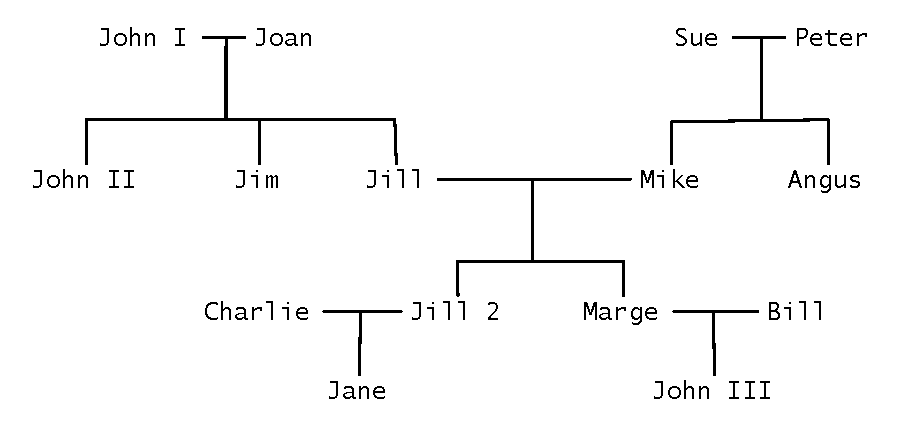
\includegraphics[width=0.8\textwidth]{familytree}}
\caption{\label{meta:tree}A family tree}
\end{figure}

We are finally in a position to put together a complete family tree and to try some queries against it. Figure~\vref{meta:tree} shows a small family tree with three generations displayed. Such a tree can be set up using the program \q{defineTree} in program~\vref{meta:family:setup}.


\begin{program}
\vspace{0.5ex}
\begin{alltt}
buildTree() ->
    Parent.assert(('John I','John II'));
    Parent.assert(('John I','Jim'));
    Parent.assert(('John I','Jill'));
    Parent.assert(('Joan','John II'));
    Parent.assert(('Joan','Jim'));
    Parent.assert(('Joan','Jill'));
    Partner.assert(('John I','Joan'));
    Partner.assert(('Peter','Sue'));
    Parent.assert(('Peter','Mike'));
    Parent.assert(('Peter','Angus'));
    Parent.assert(('Sue','Mike'));
    Parent.assert(('Sue','Angus'));
    Partner.assert(('Mike','Jill'));
    Parent.assert(('Mike','Jill 2'));
    Parent.assert(('Mike','Marge'));
    Parent.assert(('Jill','Jill 2'));
    Parent.assert(('Jill','Marge'));
    Partner.assert(('Charlie','Jill 2'));
    Parent.assert(('Charlie','Jane'));
    Parent.assert(('Jill 2','Jane'));
    Partner.assert(('Bill','Marge'));
    Parent.assert(('Marge','John III'));
    Parent.assert(('Bill','John III')).
\end{alltt}
\vspace{-2ex}
\caption{Interpreted family tree}
\label{meta:family:setup}
\end{program}

Evaluating a query against this family tree amounts to invoking the \q{satisfy()} predicate of a suitable term. For example, to list all the descendants of \q{'John I'}, we can use the forall iterator:
\begin{alltt}
(ancestor('John I',Y).satisfy() *>
  stdout.outLine("John I ancestor of "<>Y.show()))
\end{alltt}
Or to display the ancestors of \q{'Angus'}, we might use:
\begin{alltt}
(ancestor(A,'Angus').satisfy() *>
  stdout.outLine(A.show()<>"is an ancestor of Angus"))
\end{alltt}

The various labeled terms and support packages that we have introduced in this chapter mark a very convenient technique for representing interpreted programs. Of course, for a \emph{given} interpreted program, such interpretation might be over-kill -- especially for a logic program. However, the true semantics of query interpretation comes from the various implementations of \q{satisfy()} in the various classes. We can define and implement an interpreter for any language; simply by having a different kind of \q{eval}uation (say) and a similar set of support classes.

One of the nice features of the approach outlined here is the smooth integration that is possible between an interpreted program and a regular, compiled, \go program. It is straight forward for a \go program to invoke the interpreted program and similarly vice-versa.

